%%%%%%%%%%%%%%%%%%%%%%%%%%%%%%%%%%%%%%%%%%%%%%%%%%%%%%%%%%%%%%%%%%%%%%
% Lớp 10 | Hàm số bậc hai và đồ thị | Hàm số và đồ thị
% Dạng 0D3?1-5: Tính đồng biến, nghịch biến
% Số câu: 9  (sinh tự động bởi tach_cau.py; từ nay thầy sửa trực tiếp file này)
%%%%%%%%%%%%%%%%%%%%%%%%%%%%%%%%%%%%%%%%%%%%%%%%%%%%%%%%%%%%%%%%%%%%%%

%%%%%%%%%%%%%%%% TRẮC NGHIỆM 4 PHƯƠNG ÁN %%%%%%%%%%%%%%%%

% nguồn: MaHoaNH_TracNghiem_Lop10
\begin{ex}%[0D3N1-5]%[ma:1d2cc019]
	Hàm số $y=(2m+1)x+m-3$ đồng biến  trên $\mathbb{R}$ khi
	\choice 
		{\True  $m >-\dfrac{1}{2}$}
		{$m\ge-\dfrac{1}{2}$} 
		{$m  <-\dfrac{1}{2}$}
		{$m  >\dfrac{1}{2}$}
	 \loigiai{
	Hàm số đã  cho đồng biến trên $\mathbb{R} \Leftrightarrow 2m+1 > 0\Leftrightarrow m >-\dfrac{1}{2}$.}
\end{ex}

% nguồn: MaHoaNH_TracNghiem_Lop10
\begin{ex}%[0D3N1-5]%[ma:7ea2f53c]
	\immini[thm]{Hàm số bên nghịch biến trên khoảng nào?}{\begin{tikzpicture}[line cap=round,>=stealth,scale=0.7]
		\tikzset{every node/.style={scale=0.7}} 
		\draw[blue,->] (-3,0)--(3,0) node[below left] {$x$}; 
		\draw[blue,->] (0,-3.5)--(0,1) node[below left]  {$y$};
		\draw (0,0) circle (1pt) node [above  left] {$O$};
		 \draw[dashed](1,0) circle (1pt) node[above] {$1$}--(1,-1/2) circle (1pt)--(0,-1/2) circle (1pt) node[below left] {$-\dfrac{1}{2}$};
		\draw[dashed](-1,0) circle (1pt) node[above] {$-1$}--(-1,-1/2)  circle (1pt)--(0,-1/2);
		\draw[red,samples=200,domain=-2.5:2.5,smooth,variable=\x]  plot (\x,{-1/2*(\x)^2});
	\end{tikzpicture}
	 }
	\choice 
		{\True  $(0;+\infty)$}
		 {$(-1; 1)$}
		 {$(-1;+\infty)$}
		{$(-\infty;0)$} 
	\loigiai{Nhìn vào hình dáng đồ thị ta thấy hàm số  nghịch biến trên khoảng $(0; +\infty)$.
	} 
\end{ex}

% nguồn: MaHoaNH_TracNghiem_Lop10
\begin{ex}%[0D3B1-5]%[ma:d4d63084]
	 \immini{
	Cho hàm số có đồ thị như hình bên. Khẳng định nào sau  đây là đúng?
	 \choice
		{Hàm số  nghịch biến trên khoảng $(0;3)$}
		 {Hàm số đồng biến trên khoảng $(-\infty;3)$}
		{Hàm số đồng biến trên  khoảng $(-\infty;1)$}
		{\True Hàm số nghịch biến trên khoảng  $(0;2)$}}
		{\vspace{-0.5cm} 
		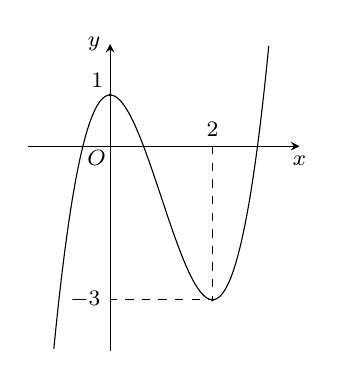
\begin{tikzpicture}[scale=0.65,font=\footnotesize,samples=200,>=stealth]
				\draw[->] (-1.6,0)--(3.7,0) node[below]{$x$}; 
				 \draw[->] (0,-4)--(0,2) node[left]{$y$};
				\node at (0,0)  [below left=-2pt]{$O$};
				\draw plot[domain=-1.1:3.1]  (\x,{(\x)^3-3*(\x)^2+1});
				 \fill
					(0,1) circle (1pt) node[above  left=-1pt]{$1$}
					(2,-3)  circle (1pt);
				 \draw[dashed]
					(2,0) node[above]{$2$} |-(0,-3)  node[left]{$-3$};
			\end{tikzpicture}
		} 
	\loigiai{ 
		Hình bên có đồ thị của hàm số đồng biến trên các khoảng $(-\infty;0)$, $(2;+\infty)$ và nghịch biến trên khoảng  $(0;2)$.
	 }
\end{ex}


%%%%%%%%%%%%%%%% ĐÚNG/SAI %%%%%%%%%%%%%%%%

% nguồn: MaHoaNH_DungSai_Lop10
\begin{ex}%[0D3N1-5]%[ma:1e820480]
	Cho hàm số $y=f(x)$ có đồ thị  là đường gấp khúc như hình dưới.
	\begin{center}
		\begin{tikzpicture}[scale=0.7,font=\footnotesize,line join=round,line cap=round,>=stealth]
				\def\xmin{-4} 
				\def\xmax{7} 
				 \def\ymin{0}
				 \def\ymax{5}
				\draw[->] (\xmin-1,0)--(\xmax+1,0) node[below] {$x$}; 
				\draw[->]  (0,\ymin-1)--(0,\ymax+1) node[left] {$y$};
				\draw (0,0) node [below left] {$O$}; 
				 \foreach \x in {-4,-3,-2,-1,1,2,3,4,5,6,7} \draw (\x,0.1)--(\x,-0.1) node [below] {$\x$};
				 \foreach \y in {1,5} \draw (0.1,\y)--(-0.1,\y) node [left] {$\y$};
				\clip  (\xmin-0.1,\ymin) rectangle (\xmax+0.1,\ymax);
				\draw  (-4,2)--(-3,0)--(-1,3)--(0,5)--(2,2)--(4,1)--(5,2)--(7,3);
				\draw[dashed]  (-4,0)|-(0,2)
					(-1,0)|-(0,3) 
					 (2,0)|-(0,2)
					(4,0)|-(0,1) 
					(5,0)|-(0,2) 
					 (7,0)|-(0,3);
				 \node[above left] at (0,2) {$2$};
				 \node[above left] at (0,3) {$3$};
			\end{tikzpicture}
	\end{center}
	Khi  đó:
	\choiceTF 
		{Tập giá trị  hàm số $T=[-4;7]$}
		 {\True Ta thấy điểm $(-4;2)$, $(4;1)$ thuộc đồ thị hàm số, điểm $(2;3)$ không thuộc đồ thị hàm số}
		 {\True Ta có $f(-1)=3$, $f(5)=2$}
		{\True Hàm số đã cho đồng biến trên các khoảng $(-3;0)$, $(4;7)$;  hàm số nghịch biến trên các khoảng $(-4;-3)$, $(0;4)$}
	\loigiai{ 
		\begin{itemchoice}
			\itemch Sai. Tập xác  định hàm số là $\mathscr{D}=[-4;7]$.\\
			Tập giá  trị hàm số là $T=[0;5]$.
			\itemch Đúng. Ta thấy điểm $(-4;2)$, $(4;1)$ thuộc đồ thị hàm số, điểm $(2;3)$ không thuộc đồ  thị hàm số.
			 \itemch Đúng. Ta có $f(-1)=3$, $f(5)=2$.
			\itemch Đúng. Hàm số đã cho đồng biến trên các khoảng $(-3;0)$,  $(4;7)$; hàm số nghịch biến trên các khoảng $(-4;-3)$, $(0;4)$.
	\end{itemchoice}}
\end{ex}

% nguồn: MaHoaNH_DungSai_Lop10
\begin{ex}%[0D3H1-5]%[ma:bb1a2cfa]
	Cho hệ bất phương trình $\heva{&  x+ y -2\leq 0 \\& 2 x-3 y +2>0}$.
	\choiceTF 
		{\True Hệ trên  là một hệ bất phương trình bậc nhất hai ẩn}
		{$\left(-1; 3\right)$ là một nghiệm của hệ bất phương trình trên} 
		 {\True $\left(1; 1\right)$ là một nghiệm của hệ bất phương trình trên}
		 {$\left(2; -2\right)$ không là một nghiệm của hệ bất phương trình trên}
	\loigiai{ 
		\begin{itemchoice}
			\itemch Hệ trên là một hệ bất  phương trình bậc nhất hai ẩn.
			\itemch Thay $x=-1; y=3$ vào hệ bất phương trình ta được $\heva{&0\ge0\\&-9>0}$ (Vô lý).\\ Vậy $\left(-1; 3\right)$ không phải là một nghiệm của  hệ bất phương trình.
			\itemch Thay $x=1; y=1$  vào hệ bất phương trình ta được $\heva{&0\le0\\&1>0}$ (luôn đúng).\\ Vậy $\left(1; 1\right)$ là một nghiệm của hệ bất phương trình.
			\itemch Thay $x=2; y=-2$ vào hệ bất phương trình ta được $\heva{&-2\le0\\&12>0}$ (luôn đúng).\\ Vậy $\left(2; -2\right)$ là một  nghiệm của hệ bất phương trình.
		\end{itemchoice}
	} 
\end{ex}

% nguồn: MaHoaNH_DungSai_Lop10
\begin{ex}%[0D3H1-5]%[ma:c8824602]
	\immini{Cho hàm số $y=f(x)$ xác định trên $\mathbb{R}$ có đồ thị như hình vẽ bên. Mỗi kết  quả dưới đây đúng hay sai?}{
	\begin{tikzpicture}[font=\footnotesize,line join=round,line cap=round,>=stealth,scale=1]
			 \draw[->] (-2,0) -- (3.5,0) node[below] {$x$};
			 \draw[->] (0,-1.2) -- (0,2.5) node[left] {$y$};
			\begin{scope}
				\clip (-2,-1.2) rectangle  (3,2.5);
				 \draw[samples=200,domain=1: 3,smooth,variable=\x] plot (\x,{(\x)-1});
				\draw[samples=200,domain=-2: 1,smooth,variable=\x] plot  (\x,{-1*(\x)+1});
			\end{scope}
			\draw[dashed]  (2,0)--(2,1)--(0,1);
			 \foreach \x/\y in{0/0,1/0,2/0,0/1,2/1,2/0}{
				\fill  (\x,\y) circle (1.5pt);
			} 
			\path 
				node at (0,0)[above left]{$O$} 
				node at  (1,0)[below left]{$1$}
				 node at (2,0)[below]{$2$}
				node at  (0,1)[left]{$1$};
		\end{tikzpicture}
	 }
	\choiceTF 
		{$f(3)=0$} 
		 {\True $f(-2)>f(0)$}
		{Điểm $\left(0;2\right)$ thuộc đồ  thị hàm số}
		 {\True $f(x)=\left|x-1\right|$}
	 \loigiai{
		\begin{itemchoice}
			\itemch Từ  đồ thị $f(3)\ne 0$.
			\itemch Do $f(-2)>f(0)$ vì hàm số  nghịch biến $\left(-\infty;0\right)$.
			\itemch Từ đồ thị của hàm số suy  ra điểm $\left(0;2\right)$ không thuộc đồ thị hàm số.
			\itemch Từ đồ thị  ta có $f(x)=\left|x-1\right|$.
		\end{itemchoice}
	 }
\end{ex}

% nguồn: MaHoaNH_DungSai_Lop10
\begin{ex}%[0D3H1-5]%[ma:c5c38282]
	Cho hệ bất phương  trình $\heva{&x+2y-100 \leq 0\\&2x+y-80\leq0\\&x\geq 0\\&y\geq 0}$.
	\choiceTF 
		{Hệ trên không phải là một hệ bất phương trình bậc nhất hai ẩn} 
		{$\left(-1; 2\right)$ là một nghiệm của hệ bất phương  trình trên}
		{\True $\left(-1; 5\right)$ không  là một nghiệm của hệ bất phương trình trên}
		{\True Miền nghiệm của  hệ bất phương trình trên là một miền tứ giác}
	 \loigiai{
		\begin{itemchoice}
			\itemch Vì hệ trên là  một hệ bất phương trình bậc nhất hai ẩn.
			\itemch Vì thay $x=-1; y=2$ vào hệ bất phương trình ta được $\heva{-97 &\leq 0\\-80&\leq0\\-1&\geq 0\\2&\geq 0} $ (Vô lý).\\ Vậy $\left(-1; 2\right)$ không phải là một nghiệm của  hệ bất phương trình.
			\itemch Thay $x=-1; y=5$ vào hệ bất phương trình ta được $\heva{&-91 \leq 0\\&-77\leq0\\&-1\geq 0\\&5\geq  0} $ (Vô lý).\\ Vậy $\left(-1; 5\right)$ không là một nghiệm của hệ bất phương trình.
			\itemch Vẽ  đường thẳng $d_1:x+2y-100=0$. Vì $0+2\cdot0-100\leq0$ nên toạ độ điểm $O\left(0; 0\right)$ thoả mãn bất phương trình $:x+2y-100\leq0$. Do đó miền nghiệm $D_1$ của bất phương trình $x+2y-100\leq0$ là nửa mặt phẳng bờ $d_1:x+2y-100=0$ chứa gốc toạ độ $O$.\\
			Tương tự miền nghiệm $D_2$ của bất phương trình $2x+y-80\leq0$ là nửa mặt phẳng bờ $d_2:2x+y-80=0$ chứa gốc toạ độ $O$.\\ 
			Tương tự miền nghiệm $D_4$ của bất  phương trình $x\geq0$ là nửa mặt phẳng bờ $Oy$ chứa điểm $\left(1; 0\right)$.\\
			Tương tự miền nghiệm $D_3$ của bất phương trình $y\geq0$ là nửa  mặt phẳng bờ $Ox$ chứa điểm $\left(0; 1\right)$.\\
			Khi đó miền nghiệm của  hệ bất phương trình là miền tứ giác $OABC$.
			\begin{center}
				\begin{tikzpicture}[scale=0.6,thick,>=stealth']
						\draw[->]  (-3,0) -- (12,0) node[above]{$x$};
						 \draw[->,color=black] (0,-2) -- (0,9) node[right]{$y$};
						\node[below left] at  (0,0) {$O$};
						\clip  (-3,-2) rectangle (12,9);
						\draw[line width=1.2pt,smooth,samples=100,domain=-1:9] plot  (\x,{-2*(\x)+8});
						\draw[line width=1.2pt,smooth,samples=100,domain=-1:15.3] plot (\x,{-0.5*(\x)+5}); 
						\fill[pattern=north east lines] (0,0)--(0,5)  --(2,4)--(4,0)-- cycle;
						\node[above]  at (4,0) {$A$};
						 \node[below] at (4,0) {$40$}; \node[below] at (10,0) {$100$};
						\node[right] at (0,5)  {$B$}; \node[left] at (0,5) {$50$};
						\node[left] at (0,8)  {$80$};
						\node[right] at (2,4)  {$C$}; \node[left] at (0,4) {$40$};
						\node[below] at (2,0) {$20$};  \draw[dashed] (0,4)--(2,4)--(2,0);
					\end{tikzpicture}
			\end{center}
		\end{itemchoice}
	} 
\end{ex}


%%%%%%%%%%%%%%%% TỰ LUẬN %%%%%%%%%%%%%%%%

% nguồn: MaHoaNH_TuLuan_Lop10
\begin{bt}%[0D3H1-5]%[ma:03516ee5]
	 Với điều kiện nào của $m$ thì hàm số $f(x)=(2m-1)x+m+3$ đồng biến trên $\mathbb{R}$? Biết kết quả có dạng $m >\dfrac{a}{b}$ (tối giản). Khi đó $2a-3b$ bằng
	\loigiai{ 
		Điều kiện để hàm số đồng biến trên $\mathbb{R}$  là $2m-1 > 0 \Rightarrow m >\dfrac{1}{2}$.\\
	Khi  đó $2a-3b=-4$.}
\end{bt}

% nguồn: MaHoaNH_TuLuan_Lop10
\begin{bt}%[0D3H1-5]%[ma:c2a2e793]
	Biểu diễn tập nghiệm của hệ bất phương trình sau trên mặt phẳng toạ độ $Oxy$? $$\heva{& 2 x+y -2>0 \\& -3x+  y-4 <0.}$$
	 \loigiai{
		\begin{itemize}
			\item Vẽ đường thẳng $\Delta_1\colon 2x+y-2=0$ đi qua hai điểm $\left(0;2\right)$ và $\left(1;0\right)$ và đường thẳng  $\Delta_2\colon -3x+y-4=0$ đi qua hai điểm $\left(0;4\right)$ và $\left(-\dfrac{4}{3};0\right)$.
			\item Xét điểm  $O(0; 0)\notin \Delta_1$. Ta có $2\cdot 0 +0 -2 =-2 <0$. Suy ra, miền nghiệm của bất phương trình $2x+y-2>0$ là nửa mặt phẳng bờ $\Delta_1$ chứa điểm $O$ không kể đường thẳng $\Delta_1$.
			\item Xét điểm $O(0; 0)\notin \Delta_2$. Ta có $-3\cdot 0 +0 -4 =-4 <0$. Suy ra, miền nghiệm của bất phương trình $-3x+y-4<0$ là nửa mặt phẳng bờ $\Delta_2$ chứa điểm $O$ không kể  đường thẳng $\Delta_2$.
		\end{itemize}
		\begin{center}
			\begin{tikzpicture}[scale=0.6,thick,>=stealth']
					\draw[->] (-3,0) --  (4,0) node[above]{$x$};
					\foreach \x  in {1,2,3}
					\draw[shift={(\x,0)},color=black] (0pt,2pt) -- (0pt,-2pt) node[below] {\footnotesize $\x$}; 
					\draw[->,color=black]  (0,-2) -- (0,6) node[right]{$y$};
					\foreach  \y in {1,2,3,4,5}
					\draw[shift={(0,\y)},color=black] (2pt,0pt)  -- (-2pt,0pt) node[left] {\footnotesize $\y$};
					\node[below  left] at (0,0) {$O$};
					\clip  (-3,-2) rectangle (4,6);
					\draw[line width=1.2pt,smooth,samples=100,domain=-3:9]  plot (\x,{-2*(\x)+2});
					\draw[line  width=1.2pt,smooth,samples=100,domain=-3:7] plot (\x,{3*(\x)+4});
					\fill[pattern=north east lines]  (-3,8)--(7,8) --(7,-12)--(2,-2)-- cycle;
					\fill[pattern=north east lines] (-3,8)--(4/3,8)  --(-2,-2)--(-3,-2)-- cycle;
				\end{tikzpicture}
		\end{center}
	 }
\end{bt}
